\documentclass[10pt,xcolor=dvipsnames]{beamer}
\usepackage{multicol}
\usetheme{Frankfurt}
%\usetheme{Bergen}
%\usetheme{Goettingen}
\usepackage{listings}
\usepackage{paralist}
\usecolortheme[RGB={0,104,139}]{structure}%deepskyblue
%\usecolortheme[named=Maroon]{structure}

\title[Cloud based IT Infra with Central Identity]{Cloud based IT Infra with Central Identity}
\subtitle{Final Presentation}

\author{ \underline{Project Guide} \\ \hspace{2mm} \\ \small{ T. Chandra Shekar } \tiny \\ \underline{} \\ \scriptsize \textit{Lecturer -- Dept. of CSE} }
\institute{ \underline{Presenting by} \\ \hspace{2mm} \\ \textit {Team r3b00+ }  \\ \hspace{4mm} \\ Dept. of CSE, RGUKT -- Nuzvid}
\usepackage{color}
 
\definecolor{codegreen}{rgb}{0,0.6,0}
\definecolor{codegray}{rgb}{0.5,0.5,0.5}
\definecolor{codepurple}{rgb}{0.58,0,0.82}
\definecolor{backcolour}{rgb}{0.95,0.95,0.92}
\lstdefinestyle{mystyle}{
    backgroundcolor=\color{backcolour},   
    commentstyle=\color{codegreen},
    keywordstyle=\color{magenta},
    numberstyle=\tiny\color{codegray},
    stringstyle=\color{codepurple},
    basicstyle=\footnotesize,
    breakatwhitespace=false,         
    breaklines=true,                 
    captionpos=b,                    
    keepspaces=true,                 
    numbers=left,                    
    numbersep=5pt,                  
    showspaces=false,                
    showstringspaces=false,
    showtabs=false,                  
    tabsize=2
}
 
\lstset{style=mystyle}

\AtBeginSection[]
{
	\begin{frame}
		\frametitle{Outline}
		\tableofcontents[currentsection,hideothersubsections]
	\end{frame}
}
%\AtBeginSubsection[] % Do nothing for \subsection*
%{
%\begin{frame}<beamer>
%\frametitle{Outline}
%\tableofcontents[currentsection,]
%\end{frame}
%}

\begin{document}


\begin{frame}
\titlepage
\end{frame}

%\begin{frame}
%\frametitle{Outline}
%\tableofcontents[hideallsubsections]
%\end{frame}

\begin{frame}{About us}

\small
\begin{center}
We are from team \textit{r3b00+}  \{reboot\} \\ \hspace{4cm} \\
\begin{tabular}{l  l }
T. Aneesh Kumar & N090247   \\
P. Nageswarao  & N091030  \\
P. Anesh  & N090977 \\
P. Jyothi Ram & N090990 \\
K. Naresh Chowdary  & N090331 \\
N. Venkata Sateesh  & N090935 \\
M. Sanyasirao & N090891  
\end{tabular}


\end{center}


\end{frame}
 

\section{Objective}
\subsection{Objective}
\begin{frame}{Objective}

Our objective is to create a  private cloud and availing access of all its services using central identity with single sign on through dynamic role based management along with REST API to third party for application developers and users. \newline

This can be developed by using open source tools like OpenStack, NFS, LDAP, Ubuntu and etc \newline

Expecting to serve with virtual machines to the research, virtual labs rather than dedicated lab hardware.
\end{frame}

\subsection{Motivation}
\begin{frame}{Motivation}

\begin{itemize}
	\item No Central Identity, Central Storage \& High capacity hardware resource pool.
	\item Failed to maintain large user load web services like ONB, Exam servers, etc.
	\item Dedicated computer course labs like Matlab, VLSI, etc.
	\item No proper Web Application Security \& Standards.
	\item Inadequate resource requirements for Research.
\end{itemize}

\end{frame}



\section{Proposed System}
\subsection{Users \& IT Services}
\begin{frame}{Users \& IT Services}
We are collaborating all IT Services that are required for University and identifing the users who is going to use them. All Users are catagorized into 4 groups $ ^{[1]}$
	
	\begin{itemize}
	\item Studens, Developers, Staff, faculty \& Researches
	\end{itemize}
\begin{figure}[H]
\begin{center}
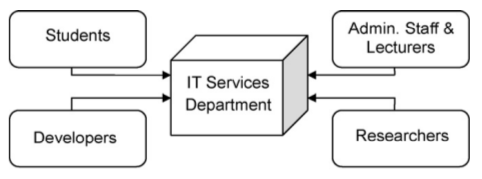
\includegraphics[width=5cm]{./it.png}
\caption{ Simplified structure of the main users of IT services. \label{fig:Simplified structure of the main users of IT services. }}
\end{center}
\end{figure}
	
\end{frame}
\subsection{Cloud Infrastructures}
\begin{frame}{Cloud Infrastructures}
All University IT Services are deployed in a private cloud, constructed over exsiting infrastructure, that can be broadly viewed as 
	
\begin{figure}[H]
\begin{center}
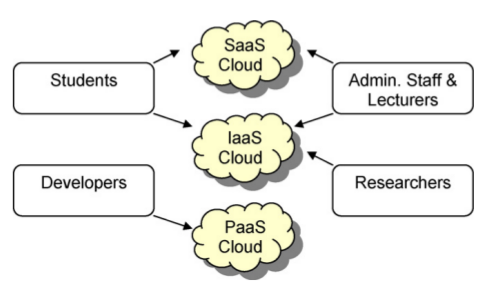
\includegraphics[width=7cm]{./it2.png}
\caption{ IT Services and Users in Cloud Computing\label{fig:IT Services and Users in Cloud Computing }}
\end{center}
\end{figure}	
	
	
\end{frame}


\section{Phase I Review}
 
\begin{frame}[allowframebreaks]{Phase I Review }
\begin{itemize}
		\item Central Identity
		\begin{itemize}
			\item Single Sign-On with REST API
			\item Fedarated Identity Management
			\item Dynamic Role Based Access Control
			\item Network Based Central Identity
			\begin{itemize}
				\item LDAP Servers
				\item NFS Servers
			\end{itemize}
		\end{itemize}
		
		\framebreak
		\item Cloud Computing
		\begin{itemize}
			\item Cloud Characterstics
			\item Service Models 
			\item Deployment Models 
			\item Private Clouds 
			\begin{itemize}
			 	\item Introduction 
				\item Open Source Tools 
			\end{itemize}	
		\end{itemize}		 
				

	\end{itemize}
\end{frame}
\section{Web Single Sign-On}

\begin{frame}
\begin{center}
\textbf{Demo}
\end{center}
\end{frame}

\subsection{OAuth Provider}
\begin{frame}{How well we implemented OAuth Provider?}
	\begin{itemize}
		\item To implement OAuth provider we used python-django and oauth-tool-kit
		\item When user requests the protected resource, oauth-tool-kit will generate client\_id and client\_secret 
		\item By using those two things user will get access\_token to access protected resource
	\end{itemize}
	  
\begin{figure}
\begin{center}
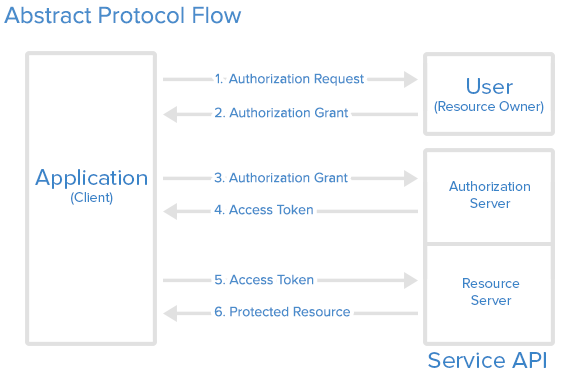
\includegraphics[width=7cm,height=3.5cm]{abstract_flow}
\caption{OAuth Protocol Work Flow Diagram\label{fig:OAuth Protocol Work Flow Diagram}}
\end{center}

\end{figure}
\end{frame}

\subsection{API Endpoints}
\begin{frame}{REST API}
	\begin{itemize}
		\item REST stands for \textbf{RE}presentational \textbf{S}tate \textbf{T}ransfer
		\item A Collection of simple URIs, and HTTP calls to those URIs and some JSON resources
		\item We implemented REST API by using django-restframework
	\end{itemize}
	\textbf{\url{/api/contact_info/?access_token=<token>}}
	\lstinputlisting[language=Java]{contact_info.json}
\end{frame}

\subsection{Testing OAuth Provider}
\begin{frame}{PHP Client Library}
\begin{itemize}
	\item We developed a Client Library for PHP Applications
	\item We used PHP-cURL to perform all the http calls and post requests to get protected data from API Server
	\item And We developed it in a modular way with Object-Oriented approach
	\item And all the function calls in the PHP library is self-explanatory
\end{itemize}
\end{frame}

\subsection{Testing OAuth Provider contd...}
\begin{frame}{PHP Client Library}
\textbf{Initializing the Client Library}
\lstinputlisting[language=php]{init.php}
\textbf{Get Authorization URL}
\lstinputlisting[language=php]{getURL.php}
\textbf{Get Access Token}
\lstinputlisting[language=php]{getToken.php}
\textbf{Initializing API with Access Token}
\lstinputlisting[language=php]{initAPI.php}
\textbf{Getting User Info from API}
\lstinputlisting[language=php]{getInfo.php}
\end{frame}
\section{Network Single SignOn}
\subsection{Introduction}
\begin{frame}{Introduction}
	Single sign-on (SSO) is a session/user authentication process that permits a user to enter one name and password in order to access multiple applications.\\
	The process authenticates the user for all the applications they have been given rights to and eliminates further prompts when they switch applications during a particular session.\\
	Components Used:
	\begin{itemize}
	\item LDAP Server
	\item phpLdapAdmin
	\item LDAP Client
	\item NFS Server
	\item NFS Client
	\end{itemize}
	
\end{frame}

\subsection{LDAP Server}
\begin{frame}{LDAP Server}
	\begin{itemize}
	\item LDAP, or Lightweight Directory Access Protocol, is a protocol for managing related information from a centralized location through the use of a file and directory hierarchy.
	\item LDAP is commonly used for centralized authentication.
	\end{itemize}
\end{frame}
\subsection{phpLDAPadmin}
\begin{frame}{phpLDAPadmin}
	\begin{itemize}
	\item Its a web-based LDAP client which provides easy, anywhere-accessible, multi-language administration for LDAP server.\\
	\item Since it is a web application, this LDAP browser works on many platforms, making your LDAP server easily manageable from any location.
	\end{itemize}
	After the installation is complete configuration will be done by making following changes in the config.php file of phpLDAPadmin.

	\lstinputlisting[language=PHP,caption=PHP Config file]{conf.php}
\end{frame}
\subsection{LDAP Client:}
\begin{frame}[allowframebreaks]{LDAP Client}
	\begin{itemize}
	\item 	LDAP-Clinet is a another droplet to act as the client machine.
	\item sudo nano \textbf{/etc/nsswitch.conf}
\end{itemize}
		The three lines we are interested in are the "passwd", "group", and "shadow" definitions. 
		Modify them to look like this:
		\lstinputlisting[language=sh,caption=Config file]{nsswitch.conf}
		\framebreak
\begin{itemize}
	\item PAM(Pluggable Authentication Modules), is a system that connects applications that can provide authentication to applications that require authentication.	\\
	\item session required \textbf{pam\_mkhomedir.so skel=/etc/skel umask=0022x}
	\item We have to add above piece of code to these files  \textbf{common-session}, \textbf{login}, \textbf{lightdm} in /etc/pam.d/ directory
	\item In order to connect to LDAP Client, we have to ssh into that particular machine.
	 \begin{itemize}
	 	\item ssh atangella@10.4.34.45
		\end{itemize}
	\end{itemize}
\end{frame}

\subsection{NFS Server}
\begin{frame}{NFS Server}
\textbf{Installation} \newline
\# apt-get install nfs-kernel-server \newline
\# mkdir -p /var/nfs \& mkdir -p /var/nfs-share \newline

\textbf{Edit /etc/exports}
\lstinputlisting[language=sh,caption=/etc/exports]{nfs.sh} 
\textbf{Exporting direcories \& Restart Server} \newline
\# exportfs -a \& \# /etc/init.d/nfsserver restart
\end{frame}

\subsection{NFS Client}
\begin{frame}{NFS Server}
\textbf{Installation} \newline
\# apt-get install nfs-client \newline

\textbf{Mounting NFS Shares} \newline
\# mount 10.4.34.201:/var/nfs-share /mnt

\end{frame}

\section{Additional Network Components}

\subsection{Introduction}
\begin{frame}{Introduction}
\begin{itemize}
 \item Maintaining fault-tolerant file systems in distributed  environment is always challenging
 \item We can achieve it through replication of data among systems
 \item But adding a load balancing on distributed systems improves response time
 \item GlusterFS provides clustered storage solution when all server systems available
 \item XtreemFS along with HAProxy helps us to achieve the goal
\end{itemize}
\end{frame}

\subsection{HAProxy}
\begin{frame}{HAProxy}
\begin{itemize}
\item HAProxy(High Availability Proxy) is an open source Reliable, High Performance TCP/HTTP Load Balancer
\item HAProxy can be configured as a front-end to load balance two VPS through private network connectivity.
\item Installing the HAProxy -- \# apt-get install haproxy
\item Configuring HAProxy 
\end{itemize}
\lstinputlisting[language=SH]{haproxy.sh}
\end{frame}

\begin{frame}{Load Balancing}
\begin{figure}[H]
\begin{center}
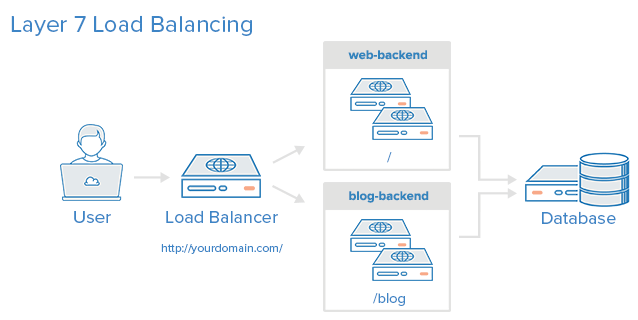
\includegraphics[width=8cm,height=4cm]{Layer7LoadBalancing.PNG}
\caption{Load Balancing }
\end{center}
\end{figure}
\end{frame}

\subsection{GlusterFS}

\begin{frame}{GlusterFS}
\begin{itemize}
\item GlusterFS is a clustered storage solution allows you to spread data in the context of a single application
\item Other systems can operate on the file system level to ensure that data is copied to another location whenever it is written to disk
\item Steps to be followed:
\begin{itemize}
 	\item  Configure DNS solution
	\item Install server components
	\item Create a storage volume
 	\item Install and configure client components
	\item Restrict access to the volume
\end{itemize}
\item  This fails in a situation where all systems are available
\end{itemize}
\end{frame}

\subsection{XtreemFS}
\begin{frame}{XtreemFS}
\begin{multicols}{2}
\begin{flushleft}

		\begin{itemize}
			\item  It’s a fault-tolerant distributed file system avails high-performance parallel access
			\item \textbf{Features:}
			\begin{itemize}
				\item  File Replication
 				\item Elasticity \& Scalability
 				\item Cloud Storage
				\item Asynchronous MRC Backup
				\item Security
				\item Stripping
			\end{itemize}

 			\item \textbf{Packages required:} xtreemfs-server, xtreemfs-client and xtreemfs-utils.
 			\item We can add replica properties and permissions to the files using xtfutils command.
		\end{itemize}

\end{flushleft}
\begin{flushright}

		\begin{figure}[H]
		\begin{center}
		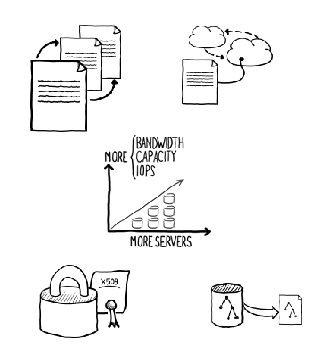
\includegraphics[width=4cm,height=4cm]{xtreem.png}
		\caption{XtreemFS Features}
		\end{center}
		\end{figure}
	

\end{flushright}
\end{multicols}
\end{frame}

\begin{frame}{XtreemFS Cont.}

\begin{figure}[H]
\begin{center}
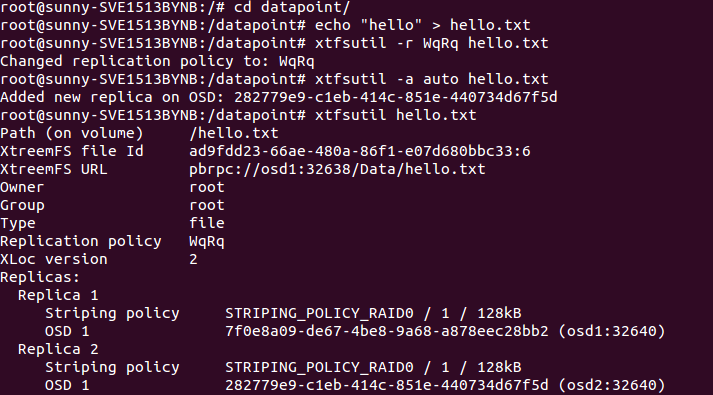
\includegraphics[width=8cm,height=6cm]{OSD1.png}
\caption{XtreemFS Distrirbuted \& Replicated Step}
\end{center}
\end{figure}

\end{frame}

\section{Additional Work}
\begin{frame}{Additional Work}
\begin{itemize}
\item Openstack Installation
\item Building Private Cloud
\item GlusterFS Replication
\item DOS Attacks on deployed Application
\end{itemize}
\end{frame}

\begin{frame}[allowframebreaks]{References}
\small
\begin{itemize}
	\item Django Docs -- \url{https://docs.djangoproject.com/en/1.7/}
	\item Django -- \url{https://djangoproject.com/}
	\item Django OAuth Tool Kit -- \url{https://github.com/evonove/django-oauth-toolkit}
	\item Django REST Framework -- \url{http://www.django-rest-framework.org/}
	\item OAuth 2.0 -- \url{http://oauth.net/2/}
	\item Semantic UI -- \url{http://beta.semantic-ui.com/}
	\item GlusterFS -- \url{https://www.digitalocean.com/How To Create a Redundant Storage Pool Using GlusterFS on Ubuntu Servers _ DigitalOcean.htm}
	\item HAProxy -- \url{www.digitalocean.com/How To Use HAProxy to Set Up HTTP Load Balancing on an Ubuntu VPS _ DigitalOcean.htm}
	\item LDAP -- \url{https://www.digitalocean.com/community/tutorials/how-to-install-and-configure-a-basic-ldap-server-on-an-ubuntu-12-04-vps}
	\item NFS Server -- \url{http://www.server-world.info/en/note?os=Ubuntu_14.04&p=nfs}
	\item NFS Client -- \url{http://www.server-world.info/en/note?os=Ubuntu_14.04&p=nfs&f=2}
	\item Openstack -- \url{http://www.server-world.info/en/note?os=Ubuntu_14.04&p=openstack_icehouse}
\item XtreemFS - \url{https://blog.headdesk.me/ Distributed filesystem with XtreemFS _ xpk's blog.htm}
\end{itemize}
\end{frame}



\begin{frame}{End}
Thank you and Any Queries ?
\end{frame}

\end{document}